\section{Process Analysis}
\label{process-analysis}

\paragraph{Research with the \project{} dataset}
When doing research in the medical domain a well known workflow is often used. Nwogu \cite{nwogu} has formally described and defined this workflow for scientific reporting purposes (\ie{} writing scientific papers).
The {\tt Research Workflow} in figure \ref{fig:research-workflow} shows the simplification of this workflow, which includes problem definition, formulation of research question, definition of methods, data aquisition, statistical analysis, analysis results, and conclusion.

Clinical research (\eg{} a trial) is well suited to follow this workflow, as each step can be executed in turn.
Of these steps data acquisition is often the most time-consuming part.
However, acquisition of new data is not always necessary,  desirable or even possible. 
Research data of high quality and trustworthiness is valuable and should be preserved and re-used, under well controlled conditions. 
This is also the case with the \projectdata{}.

The goal of the proposed \ivfsystem{} is to facilitate reuse of this data.
There is, however, one major restriction with data sharing and re-use: medical data is (almost always) highly sensitive and must be secured. 
This imposes strong conditions for reusing the data, which have to be taken into account by the system.

For reuse purposes three actors are important: researcher, data manager, and interested third parties (\eg{} clinics, public, government).
Researchers are actors interested in analysis of the \projectdata{} for scientific ends.
The data manager is the central point of communication for everything that has to do with the dataset, but is also responsible for keeping an overview of everything that happens during the steps in the process.
Lastly, third parties are actors interested in research conclusions and possibly aggregated (statistical) data from the \projectdata{}.

Currently when a dataset like the \projectdata{} is exploited for reuse the following happens.
A researcher asks what data is available and can search to find what he/she needs.
Then a data request is formulated and a permission granting process is initiated.
A request contains the necessary information to base a permission decision on, \eg{} problem background, research question, and perceived methods to answer question.
The research committee evaluates the request and based on this the researcher gets permission to receive data.

At a first look it seemed the system would boil down to data acquisition.
As addition to wrapping this process into a system the execution of analysis and storing the results was added to boost the usefulness for researchers.
The acquisition and analysis processes overspan a big chunk of the research workflow, which is depicted in figure \ref{fig:research-workflow} with the gateway function groups.

\begin{figure}[t]
	\centering
	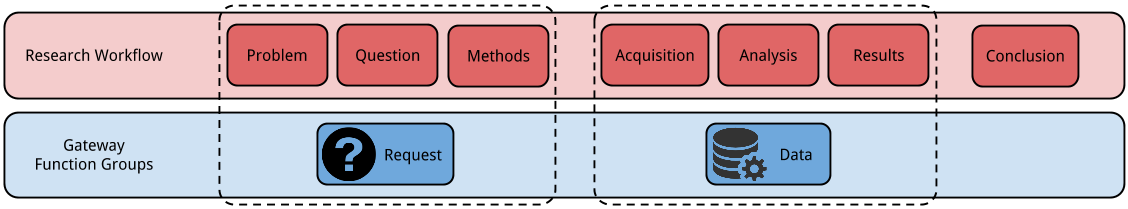
\includegraphics[width=1.0\linewidth]{images/research-workflow}
	\caption{
		This figure shows a simplification of the research workflow often used  in the medical domain (based on Nwogu \cite{nwogu}).
		The workflow components are mapped (dotted lines) by the identified \ivfsystem{} function groups.
		Note: the data acquisition component requires execution of acquisition methods defined in the methods component. \allard{remove note?}
	}
	\label{fig:research-workflow}
\end{figure}